In the forthcoming deployment of WebRTC systems, we speculate that high
quality\footnote{normally, corresponds to increase in required bandwidth}
video confrencing will see wide adoption. Normally, to assure stability of the
network (and avoid congestion collapse), these real-time communication systems
will need to implement some kind of congestion control for their RTP-based
media traffic.

RTP transmits the media data over IP using a variety of transport layer
protocols such as UDP, TCP, and Datagram Congestion Control Protocol (DCCP).
Consequetly, congestion control for RTP-based media flows can be implemented
either in the application or the media flows are transmitted over congestion-%
controlled transport (TCP or DCCP). While using a congestion controlled
transport may be safe for the network, it is suboptimal for the media quality
unless the congestion-controlled transport is designed to carry media flows or
operates in a very low latency network ($<100$ms)~\cite{Brosh:tcp-real-time}.
On the other hand, using a non-congestion controlled transport (e.g., UDP),
the rate-adaptation is implemented in the application.  In this thesis, we
consider congestion control for unicast RTP traffic running over best-effort
IP network.

% CC should not cause queuing delay. Or define low-delay operation of
% multimedia cc.

\section{RTCP Reporting Interval}

Endpoint needs to rely on RTCP feedback from the receiver to implement
congestion control.  Additionally, the congestion control algorithm needs to
be aware of the limits on the timing of the feedback. 

% per-packet, per-frame, per-RTT

but unlike other delay-based variants of TCP there
may not be sufficient RTCP bandwidth to provide feedback on a per-packet
basis~\cite{draft.rmcat.feedback}.



\section{Framework for Congestion Cues}
\label{fw.fw}


\begin{figure}
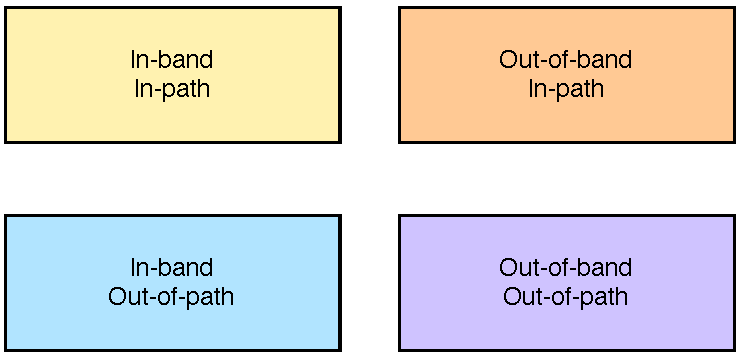
\includegraphics[scale=1.0]{chap2-fw-outline}
\caption{Congestion Cue Framework}
\label{fig:4:fw}
\end{figure}


\section{Requirements for Congestion Control}
\label{fw.cc.req}

\section{Framework for Evaluating Congestion Control}
\label{fw.cc.eval}

% Flow scenarios
% Link properties
% Router properties